\documentclass[12pt]{extarticle}
\usepackage{tikz}
\usepackage{amsmath,amssymb}
\usepackage{caption}
\usepackage{graphicx}
\usepackage{multicol}
\usepackage{hyperref}
\usepackage{geometry}
\usepackage{watermark}
\usepackage{varwidth}
\usepackage{float}
\usepackage{arydshln}
\usepackage[dvipsnames]{xcolor}
\usepackage{tcolorbox}
\usepackage{booktabs}
%\usepackage{scrlayer-scrpage}
\usepackage{forest}
\usepackage{fancyhdr}
\pagecolor{white}
\geometry{bottom= 30mm}
\usepackage{enumitem}


\newcommand{\assignnumber}{\color{red}number\color{black}} %tell latex number of Homework

\title{Data Management Assignment 6}
\author{Cuihuan Zhang} 
\fancyhead[L]{Data Management}
\fancyhead[C]{Assignment 6}
\fancyhead[R]{Cuihuan Zhang}
\renewcommand\headrulewidth{0pt}
\pagestyle{fancy}
\pagenumbering{arabic}

\begin{document}

\maketitle \vspace{-10mm}
\rule{\linewidth}{0.4pt}

\begin{flushleft}
\begin{enumerate}

\item

\begin{enumerate}

\item \begin{tabular}{cll}
\toprule
\textbf{Database items} & \textbf{Operation} \\
\midrule
T1     & Not affected by the failure   \\
T2     & Not affected by the failure    \\
T3     & Undo    \\
T4     & Redo   \\
T5     & Undo   \\
T6     & Undo   \\
\bottomrule
\end{tabular}

\begin{enumerate}

\item T4 needs to be Redo, since T4 is committed after the checkpoint.
\item Obviously, T3, T5 and T6 are uncommitted items, so we need to Undo them.
\item T1 and T2 are not affected by the failure since T1 and T2 are committed before the checkpoints. The modifications of T1 and T2 have been persisted to the disk through checkpoints.
\end{enumerate}

\item

\begin{enumerate}
\item
\begin{tabular}{cll}
\toprule
\textbf{Database items} & \textbf{Possiable values} \\
\midrule
a     & 1 or 2   \\
b     & 2 or 3    \\
c     & 0 or 1    \\
\bottomrule
\end{tabular}

\item
\begin{tabular}{cll}
\toprule
\textbf{Database items} & \textbf{Possiable values} \\
\midrule
a     & 2   \\
b     & 2    \\
c     & 0    \\
\bottomrule
\end{tabular}
\end{enumerate}

\end{enumerate}

\item

\begin{enumerate}
\item

\begin{enumerate}
\item Recoverable: In a scheduling, if transaction T' reads the modified data of another transaction T, then the commit of transaction T' must occur follow the commit of transaction T.
\item Cascadeless (no cascading aborts): If transaction T' reads only values produced by transaction T that have already committed.
\item Strict: if 1. satisfies the condition for avoiding cascading aborts and 2. for every transaction, if it writes an item, all the transactions that previously wrote that item have already committed or aborted.
\end{enumerate}

\item

\begin{enumerate}
\item
Recoverable: This schedule is recoverable. T5 reads the value z after the commit of T3. Although T2 haven't committed x, but T4 also haven't committed yet.\\
Cascadeless (no cascading aborts): T4 violated cascadeless. T4 reads the value x that have not already committed by T2. \\
Strict: T4 violates strictness. Since it is not satisfies the condition for avoiding cascading aborts.\\

\item
Recoverable: This schedule is not recoverable. T4-read(b) have been committed before T1-write(b), so T4 violated recoverable.\\
Cascadeless (no cascading aborts): T4 violated cascadeless. T4-read(b) reads b that have not committed by T1-write(b).\\
Strict: T1, T2 and T4 violates strictness. T1 writes b before T2 committed write(b) (T1 write b overwrites the uncommitted b in T2) and same problem for c. And it is obvious that  T4 does not satisfied the condition for avoiding cascading aborts.\\
\end{enumerate}

\end{enumerate}

\item

\begin{enumerate}

\item The schedule is serializable (no cycle), the serial equivalent can be [T1, T3, T5, T2, T4] or [T3, T5, T1, T2, T4] or [T3, T1, T5, T2, T4].\\
\item The schedule is not serializable, in any order of [T1, T2, T4, T3, T5], [T2, T1, T4, T3, T5] etc. Always a conflict between [T1, T2] since it is a cycle. \\
Note: conflict graphs and examples are on the next page.

\begin{figure}[h]
  \centering
  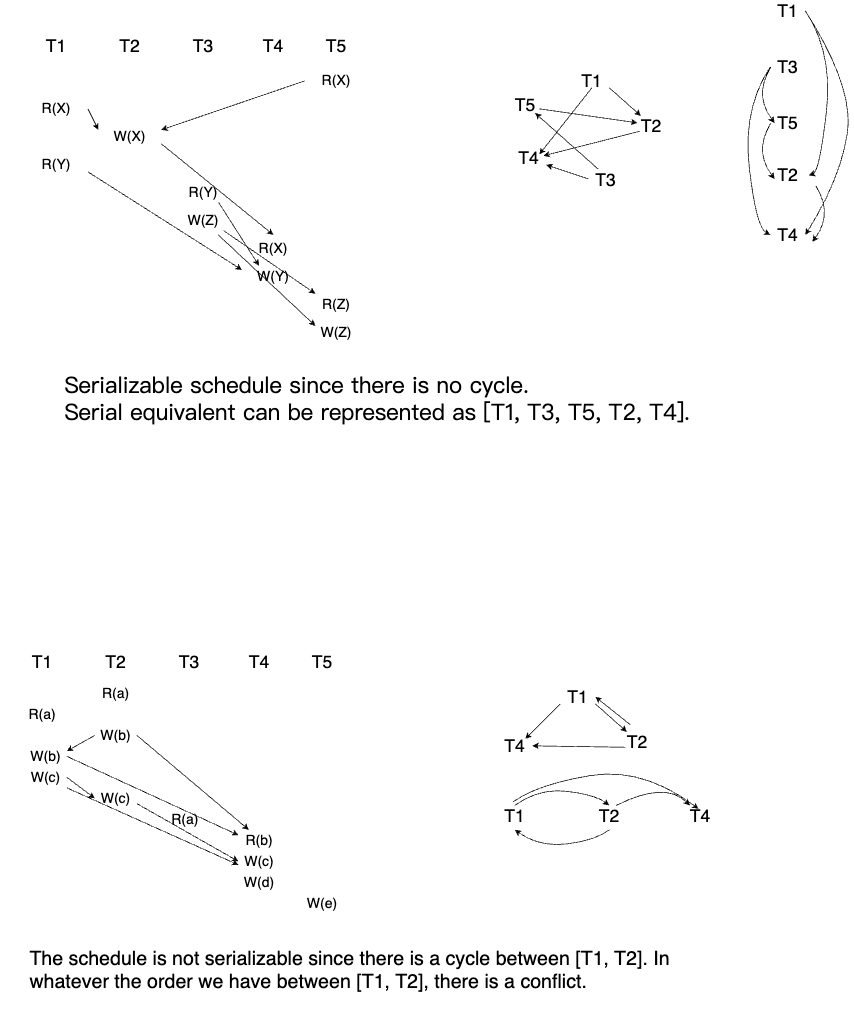
\includegraphics[width=0.8\textwidth]{hw6_c.drawio.png}
  \caption{Serializability of concurrent transactions}
\end{figure}

\end{enumerate}

\end{enumerate}
\end{flushleft}
\end {document}